\documentclass{article}
\usepackage{amsmath, fullpage}
\usepackage[portuguese]{babel}
\usepackage{graphicx}
\usepackage{color}
\usepackage{subcaption}
\usepackage{listings}
\usepackage{amssymb}
\usepackage[thmmarks]
{ntheorem}
\usepackage{booktabs}
\usepackage{mdframed}
\graphicspath{{imgs/}}

\begin{document}

\newcounter{boxlblcounter}  
\newcommand{\makeboxlabel}[1]{\fbox{#1.}\hfill}% \hfill fills the label box
\newenvironment{boxlabel}
  {\begin{list}
    {\arabic{boxlblcounter}}
    {\usecounter{boxlblcounter}
     \setlength{\labelwidth}{3em}
     \setlength{\labelsep}{0em}
     \setlength{\itemsep}{2pt}
     \setlength{\leftmargin}{1.5cm}
     \setlength{\rightmargin}{2cm}
     \setlength{\itemindent}{0em} 
     \let\makelabel=\makeboxlabel
    }
  }
{\end{list}}

\newenvironment{boxedd}
    {
     \begin{center}
    \begin{tabular}{|p{1\textwidth}|}
    \hline
    }
    { 
    \\\\\hline
    \end{tabular} 
    \end{center}
    }



 

\title{Introdução aos processadores programáveis}
\author{Henrique Bernardes}
%\date{\vspace{-5ex}}
\maketitle
\thispagestyle{empty}

\section{Início - Arquitetura básica de um processador programável}
%\fbox{textInsideBox}
%\colorbox{red}{coloredText}
%\scalebox{6}[7]{bigText}
Começamos aqui esclarecendo as diferenças entre hardware dedicado e um processador de propósito geral, tendo como objetivo diferenciar o que estávamos trabalhando do que vamos passar a trabalhar.

Um hardware dedicado implementa circuitos digitais para realizar uma determinada tarefa, podendo assim ser costumizado. Além disso, principalmente pela capacidade de paralelização, hardware dedicado tem um alto desempenho. Contudo, apresenta alto custo e pouca flexibilidade, uma vez que qualquer alteração reflete uma modificação no circuito. 

Já um processador de propósito geral tem seu "programa" armazenado em memória, podendo ser modificado, uma vez que se baseia em software, acarretando, também, em um menor tempo de desenvolvimento. Contudo, pelo fato de aqui termos uma sequência de instruções ao invés de um fluxo de dados, é difícil paralelizar o algoritmo, apresentando um baixo desempenho. Dentre os diversos processadores de propósito geral podem ser listados os Intel, AMD, ARM, MIPS e ATMega.

\begin{figure}[h!] 
    \centering 
    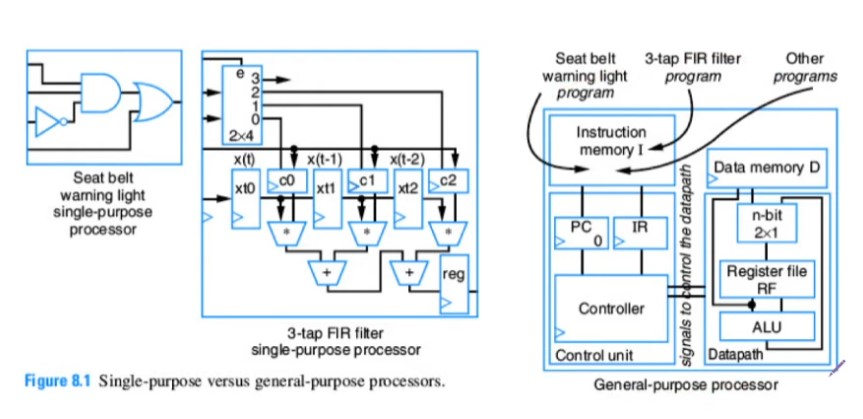
\includegraphics[width=1\textwidth]{imgs/x.jpg} 
    \caption{Hardware dedicado versus processador de propósito geral} 
    \label{fig:comparacao1} 
\end{figure}

\newpage
\section{Arquitetura load-store}
\subsubsection{Caminho de dados}

A memória de dados armazena todos os dados que o processador pode acessar. Esses dados devem passar pelo banco de registradores antes de ser processados pela Unidade Lógica Aritmética(ULA), armazenando os dados a serem operados pela ULA. Ao longo do caminho, o multiplexaddor 2x1 escolhe entre os dados da memória ou os resultados intermediários da ULA.

\begin{figure}[h]
\centering
\begin{minipage}{0.48\textwidth}
     \centering
     \def\svgwidth{0.7\textwidth}
     \input{imgs/selmux.eps_tex}
     \caption{\label{fig:loadstore} Caminho de dados de uma arquitetura load-store. }
     \hfill
\end{minipage}\hfill
\begin{minipage}{0.48\textwidth}
    \centering 
    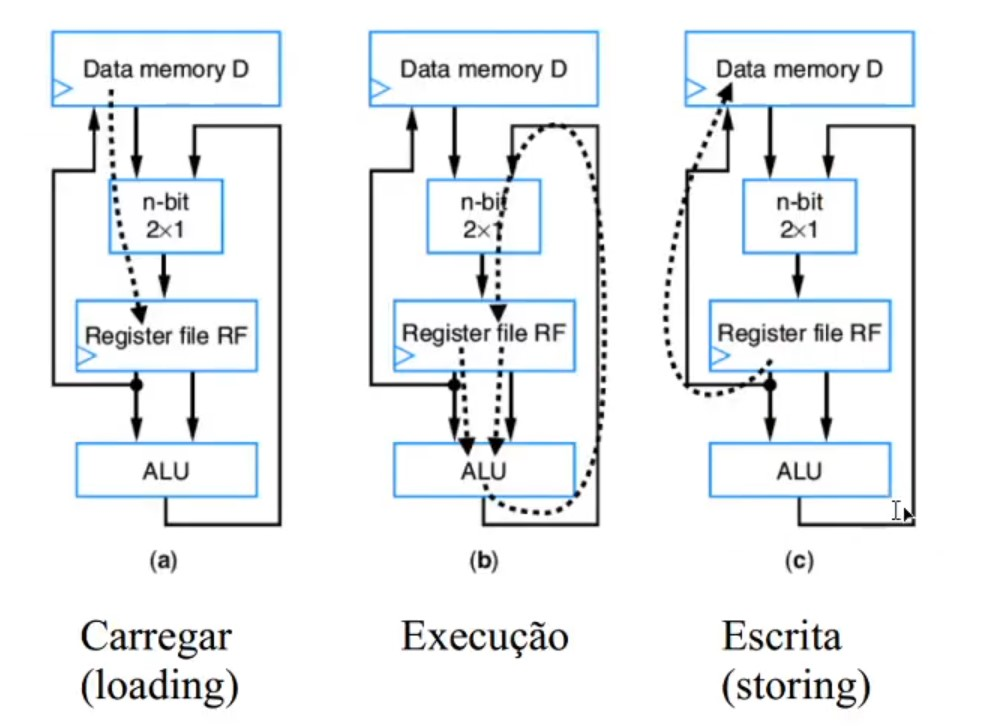
\includegraphics[width=1\textwidth]{loadstore2.jpg} 
    \caption{Casos de carregação, execução e escrita de dados em uma arquitetura load-store} 
    \label{fig:casosloadstore} 
\end{minipage}
\end{figure}


Ou seja, o processamento ocorre por meio destas três instruções (figura \ref{fig:casosloadstore}):

\begin{boxlabel}
     \item Carregar dados - leitura de um determinado \textit{address} e carregamento no banco de registradores;
     \item Transformar dados - executar operações;
     \item Armazenar dados - escrita - um resultado intermediário vindo da ULA pode ser enviada de volta para a memória de dados (também, para o endereço  \textit{address})
\end{boxlabel}

\newpage
\subsubsection{Unidade de Controle}
A unidade de controle está para o caminho de dados como uma FSM, de fato, como é de se esperar, ela controla o caminho de dados; ou seja, nesta unidade são configurados os sinais de \textit{clear}, \textit{load}, \textit{addresses} da memória de dados e do banco de registradores e seleção do multiplexador.

\begin{figure}[h!]
     \centering
     \def\svgwidth{0.4\textwidth}
     \input{imgs/fdx.eps_tex}
     \caption{\label{fig:fdx} Unidade de controle básica. }
     \hfill
\end{figure}

Inicialmente, a unidade lê as instruções da memória de instruções I.

Em uma arquitetura FDx de três estágios, as intruções são realizadas em uma média total de três ciclos de clock, baseadas em três componentes: 
\begin{itemize}
     \item PC (\textit{program counter}): Contador que indica a próxima instrução a ser lida;
     \item IR (\textit{instruction register}): Armazena a instrução;
     \item Controlador(\textit{Controller}): FSM
\end{itemize}
As operações são descritas abaixo:

\begin{boxlabel}
     \item Busca (\textit{\textbf{F}etch}): Lê I[address] e armazena no registrador local IR(\textit{instruction register});
     \item Decodificação (\textit{\textbf{D}ecode}): Determina a operação a ser executada;
     \item Execução (\textit{E\textbf{x}ecute}): Gera os sinais de controle para o caminho de dados de modo que a instrução seja executada.
\end{boxlabel}

A figura \ref{fig:fdx2} demonstra a interface entre o \textit{controller}(FSM) e o resto da unidade:

\newpage
\begin{figure}[h!]
     \centering
     \def\svgwidth{0.7\textwidth}
     \input{imgs/fdx2.eps_tex}
     \caption{\label{fig:fdx2} Interface entre os elementos na unidade de controle e a FSM em si.}
     \hfill
\end{figure}



Temos como exemplo a seguinte operação a ser realizada: 
$ D[9]=D[0]+D[1] $
 
\begin{minipage}{0.48\textwidth}
     \begin{lstlisting}
          RF[0]=D[0]     - load
          RF[1]=D[1]     - load
          RF[2]=RF[0]+RF[1] - (ULA)
          D[9]=RF[2]     - write
     \end{lstlisting}    
\end{minipage}
\begin{minipage}{0.48\textwidth}
     
     .\\
     .\\
     .\\
     .\\
     $\rightarrow$ Aqui, o valor na posição 2 do register file é escrito na posição 9 do data memory.
      
\end{minipage}
 
Na figura \ref{fig:unidadeControleExemplo} observa-se a primeira linha se propagrando ao longo da unidade de controle e caminho de dados


\begin{figure}[h]
\centering
\begin{minipage}{0.48\textwidth}
     \centering
     \def\svgwidth{0.4\textwidth}
     \input{imgs/fdx3.eps_tex}
     \caption{\label{fig:fdx3} Instruções e armazenamento no \textit{instruction memory I}.}
     \hfill
\end{minipage}\hfill
\begin{minipage}{0.48\textwidth}
    \centering 
    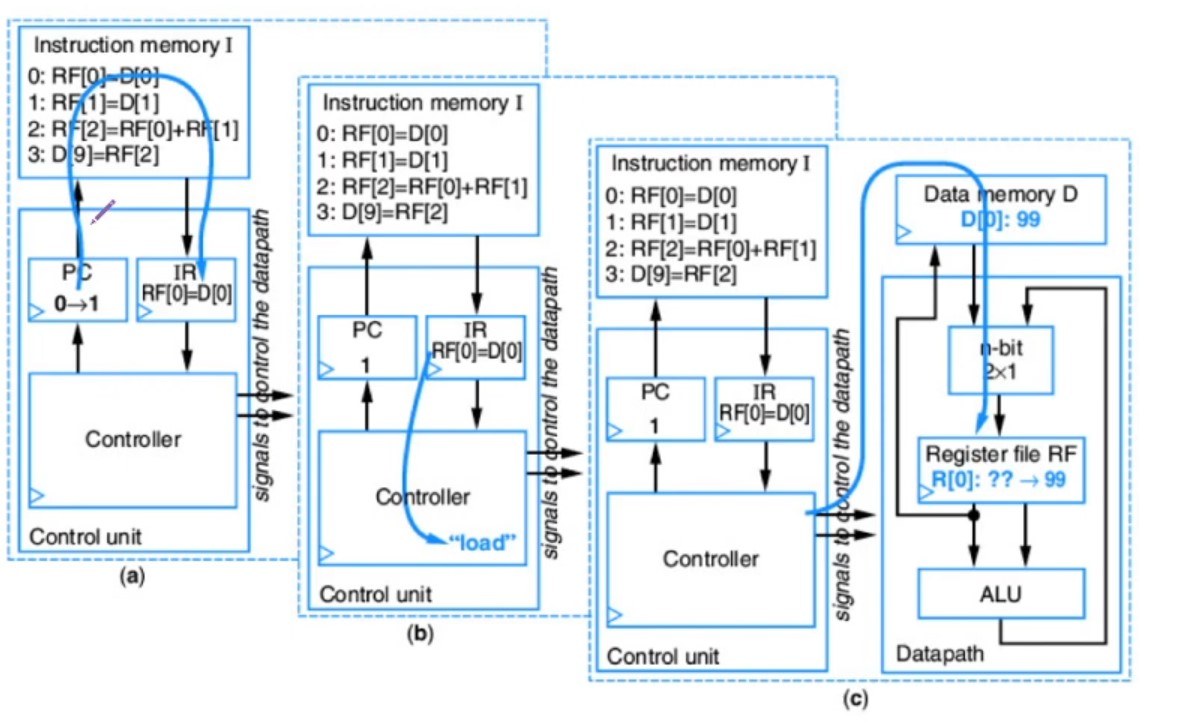
\includegraphics[width=1\textwidth]{unidadeControle.jpg} 
    \caption{Primeira linha de código se propagando pela unidade de controle e caminho de dados.} 
    \label{fig:unidadeControleExemplo} 
\end{minipage}
\end{figure}

\iffalse
Given a sequence of $n$ points in the plane $(X_1, Y_1), \ldots, (X_n, Y_n)$
we seek the linear equation $y = a + bx$ that approximates the points
as closely as possible, in the sense that the sum of the squared residuals
$E = \sum_{i=1}^n (Y_i - a - bX_i)^2$ is minimized.

We assume that not all of the points lie on a single horizontal or vertical
line. In that case, we can apply a \emph{transformation} to the points
so that $\sum x_i = \sum y_i = 0$ and $\sum x_i^2 = \sum y_i^2 = 1$.
The transformation is defined by
$$
x_i = \frac{X_i - \overline{X}}{\sqrt{\sum (X_i - \overline{X})^2}}\quad\text{and}\quad
y_i = \frac{Y_i - \overline{Y}}{\sqrt{\sum (Y_i - \overline{Y})^2}}.
$$

This transformation is linear, so it maps lines to lines.
If we transform a line fitted to the data,
the sum of squared residuals is multiplied by a positive constant factor.
Therefore, the transformation preserves the line of best fit.


Let $r = \sum x_i y_i$. Then
\begin{align*}
E &= \sum (y_i - a - bx_i)^2 \\
&= \sum (y_i^2 + a^2 + b^2 x_i^2 - 2ay_i - 2bx_iy_i + 2abx_i) \\
&= \sum y_i^2 + \sum a^2 + \sum b^2 x_i^2 
 - \sum 2ay_i - \sum 2bx_iy_i + \sum 2abx_i \\
&= 1 + na^2 + b^2 - 2br \\
&= (1-r^2) + na^2 + (b - r)^2\ .
\end{align*}

The sum is minimized when $a = 0$ and $b = r$, so the line of best fit is
$y = rx$. What a simple equation!
Unfortunately, the equation is a bit messier when expressed in terms of the
original variables.

\begin{align*}
\frac{y - \overline{Y}}{\sqrt{\sum (Y_i - \overline{Y})^2}}
&= \left(
     \frac{\sum (X_i - \overline{X}) (Y_i - \overline{Y})}
          {\sqrt{\sum (X_i - \overline{X})^2 \sum (Y_i - \overline{Y})^2}}
   \right)
   \left(
     \frac{x - \overline{X}}
          {\sqrt{\sum (X_i - \overline{X})^2}}
   \right)\\
y - \overline{Y} &=
\left(
     \frac{\sum (X_i - \overline{X}) (Y_i - \overline{Y})}
          {\sum (X_i - \overline{X})^2}
   \right)
   (x - \overline{X})\ .
\end{align*}

Note that $r$ is the Pearson correlation coefficient of the sample.
This shows that the correlation coefficient can be interpreted geometrically
as the slope of the line of best fit when the $x$ and $y$ values are standardized.
\fi

\newpage
\section{Processador programável  de três instruções}
Inicialmente, definimos o que é conhecido como \textbf{conjunto de instruções} do processador programável: é uma lista das instruções possíveis e a meneira de representar essas instruções na memória.
Vamos definir, também, que um processador usa instruções de 16 bits e que a memória de instruções I tem 16 bits de largura. Normalmente, um determinado número de bits é reservado pelo conjunto de instruções para indicar a instrução em si a ser realizada sendo que os restantes especificam informações adicionais como registradores de origem, destino, etc.

Definiremos um conjunto de três operações símples, onde os 4 bits mais significativos irão representar a operação e os 12 restantes indicam os endereços no banco de registradores(\textit{register file}) e na memória de dados.

Teremos, então, as seguintes instruções:


\begin{boxedd}
\begin{lstlisting}
(0) Carregar - load - 0000(r3)(r2)(r1)(r0)(d7)(d6)(d5)(d4)(d3)(d2)(d1)(d0)
(1) 0000 0000 00000000
(2) 0000 0001 00101010
\end{lstlisting}    
Esta instrução especifica uma movimentação de dados que vai de uma posição da memória de dados(especificado pelos $d_i$ bits) até um registrador no banco de registradores(especificado pelos $r_i$ bits), ou seja, funciona como uma instrução de \textit{fetch}.\\
Como exemplo, primeiro, a linha 1 indica uma operação de movimentação de dados do da posição 0 da memória de dados($D[0]$) até a posição 0 do banco de registradores($RF[0]$), ou seja, esta instrução realiza a operação $RF[0]=D[0]$. 

A linha 2 indica uma operação de movimentação de dados da posição 42 da memória de dados ($D[42]$) até a posição 1 do banco de registradores ($RF[1]$). Ou seja, especifica a operação $RF[1]=D[42]$
\end{boxedd}
 

\begin{boxedd}
\begin{lstlisting}
(0) Armazenar - store -0001(r3)(r2)(r1)(r0)(d7)(d6)(d5)(d4)(d3)(d2)(d1)(d0)
(1) 0001 0000 00001001
\end{lstlisting}    
Essa instrução especifica uma movimentação de dados no sentido oposto da instrução anterior, indo do banco de registradores até a memória de dados, ou seja, funciona como uma instrução de \textit{store}. \\
Assim sendo, a instrução da linha 1 armazena no endereço 9 da memória de dados ($D[9]$) o dado que está localizado no endereço 0 do banco de registradores($RF[0]$).
\end{boxedd}
 
\begin{boxedd}
\begin{lstlisting}
(0) Somar-add-0010(ra3)(ra2)(ra1)(ra0)(rb3)(rb2)(rb1)(rb0)(rc3)(rc2)(rc1)(rc0)
(1) 0010 0010 0000 0001
\end{lstlisting}    
Essa instrução especifica somar os conteúdos de dois registradores do banco de registradores, especificados por $rb_3 rb_2 rb_1 rb_0$ e $rc_3 rc_2 rc_1 rc_0$ e então armazenar no registrador do banco de registradores especificado por $ra_3 ra_2 ra_1 ra_0$.\\
Assim sendo, a instrução da linha 1 especifica somar o conteúdo do registrador $RF[0]$ ao conteúdo do registrador $RF[1]$ e armazenar no registrador $RF[2]$, ou seja, $RF[2] = RF[0] + RF[1]$.
\end{boxedd}

Nenhuma dessas operações modifica os conteúdos dos operandos de origem, ou seja:
\begin{itemize}
     \item A instrução \textbf{carregar} faz com que os conteúdos de um endereço da memória  de dados $D[i]$ sejam carregados em um registrador do banco de registrador $RF[i]$, sem alterar o conteúdo naquele endereço da memória de dados $D[i]$.
     \item A instrução \textbf{armazenar} faz com que os conteúdos de um endereço do banco de registrador $RF[i]$ sejam armazenados em um endereço da memória de dados $D[i]$ sem alterar o conteúdo daquele registrador $RF[i]$.
     \item A instrução \textbf{somar} faz com que os dados dos registradores $Rb[i]$ e $Rc[i]$ sejam somados e armazenados em $Ra[i]$ sem alterar os conteúdos dos registradores  $Rb[i]$ e $Rc[i]$.
\end{itemize}

Assim sendo, é possível entender o processo para realizar a operação $D[9]=D[0]+D[1]$ (figura \ref{fig:OperaçãoD9D0D1}):
\begin{boxedd}{OPERAÇÃO D[9]=D[0]+D[1]}
     \begin{lstlisting}
     (0) load - RF[0] = D[0] - 0000 0000 00000000
     (1) load - RF[1] = D[1] - 0000 0001 00000001
     (2) add - RF[2]=RF[0]+RF[1] - 0010 0010 0000 0001
     (3) store - D[9] = RF[2] - 0001 0010 00001001
     \end{lstlisting}  
\end{boxedd}

\begin{figure}[h!] 
    \centering 
    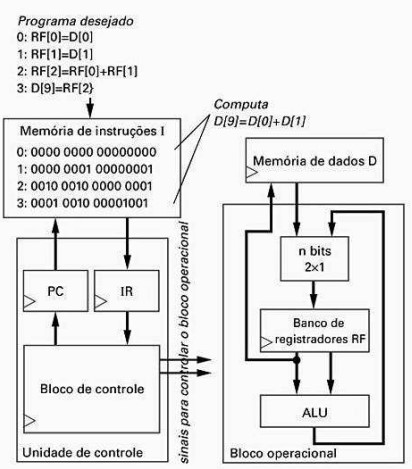
\includegraphics[width=0.5\textwidth]{d9equalsd0plusd1.jpg} 
    \caption{$D[9]=D[0]+D[1]$} 
    \label{fig:OperaçãoD9D0D1} 
\end{figure}

Realizando a operação $D[5]=D[5]+D[6]+D[7]$:


\begin{boxedd}{OPERAÇÃO D[5] = D[5] + D[6] + D[7]:}
     \begin{lstlisting}
(0) 0000 0000 00000101   // load  -  RF[0] = D[5] 
(1) 0000 0001 00000110   // load  -  RF[1] = D[6] 
(2) 0000 0010 00000111   // load  -  RF[2] = D[7] 
(3) 0010 0011 0000 0001  // sum   -  RF[3] = RF[0]+RF[1] ou D[5]+D[6]
(4) 0010 0011 0011 0010  // sum   -  RF[3] = RF[3]+RF[2] ou D[5]+D[6]+D[7]
(5) 0001 0011 00000101   // store -  D[5]  = RF[3]

otimizando para utilizar apenas 3 registradores do banco de registradores

(0) 0000 0000 00000101   // load  -  RF[0] = D[5] 
(1) 0000 0001 00000110   // load  -  RF[1] = D[6] 
(2) 0000 0010 00000111   // load  -  RF[2] = D[7] 
(3) 0010 0011 0000 0001  // sum   -  RF[0] = RF[0]+RF[1] ou D[5]+D[6]
(4) 0010 0011 0011 0010  // sum   -  RF[0] = RF[0]+RF[2] ou D[5]+D[6]+D[7]
(5) 0001 0011 00000101   // store -  D[5]  = RF[0]
     \end{lstlisting}    
\end{boxedd}


Finalmente, como foi visto, na memórias de instruções, as instruções existem como sequências de 0s e 1s, representação denominada como \textbf{código de máquina}. Como é de se esperar, escrever um programa inteiro dessa forma acarretaria em muitos erros. Por esse motivo, utiliza-se uma ferramenta chamada \textit{assembler}, que permite escrever instruções usando mnemônicos, ou símbolos, que o \textit{assembler} traduz para código máquina. Um código escrito em mnemônicos é chamado de \textbf{código assembly}.
Dessa forma, no contexto do conjunto de três instruções, um \textit{assembler} nos permite escrever as instruções usando os seguintes mnemônicos:

\begin{boxlabel}
     \item Carregar - MOV Ra, d - especifica a operação $RF[a] = D[d]$. O valor de $a$ pode assumir quaisquer valor de 0 a $2^{4}-1$, ou seja, 0 a 15, assim, R0 significa $RF[0]$, R1 significa $RF[1]$, etc. O valor de $d$ pode assumir quaisquer valor de 0 a $2^{8}-1$, ou seja, 0 à 255.
     \item Armazenar - MOV d, Ra - especifica a operação $D[d]=RF[a]$;
     \item Somar - ADD Ra, Rb, Rc - especifica a operação $RF[a]=RF[b]+RF[c]$
\end{boxlabel}

Com o uso desses mnemônicos o programa $D[9]=D[0]+D[1]$ pode ser rescrito como:

\begin{boxedd}{OPERAÇÃO D[9]=D[0]+D[1]:}
     \begin{lstlisting}
(0) MOV R0, 0
(1) MOV R1, 1
(2) ADD R0, R0, R1
(3) MOV 9, R0
     \end{lstlisting}    
\end{boxedd}

\newpage
Tendo estabelecido a base dos processadores de três instruções, como suas instruções e a arquitetura básica, podemos expandir o bloco fsm da figura \ref{fig:fdx2}, principalmente, o estado \textit{execute}.

\begin{figure}[h!] 
    \centering 
    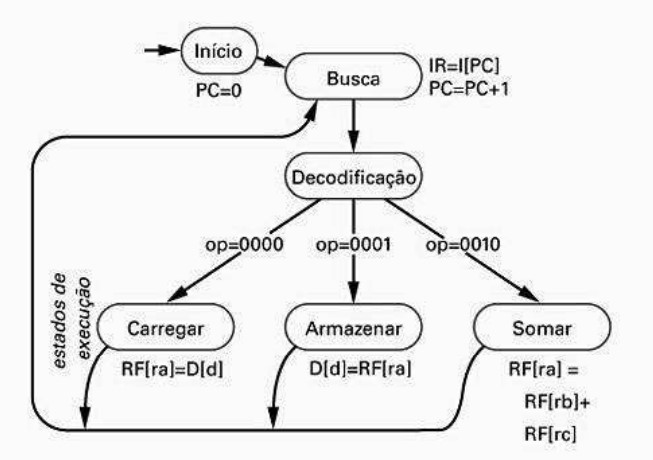
\includegraphics[width=0.8\textwidth]{fsmExpandida.jpg} 
    \caption{FSM com estado execute expandido.} 
    \label{fig:fsmExpandida} 
\end{figure}

Primeiramente, assumimos que op é uma abreviação de $IR[15...12]$, ou seja, os bits mais significativos do \textit{instruction register}. O mesmo pode ser dito sobre ra($IR[11...8]$), rb($IR[7...4]$), rc($IR[3...0]$) e d($IR[7...0]$), ou seja:
\begin{itemize}
     \item op $ \rightarrow  IR[15...12]$
     \item ra $ \rightarrow IR[11...8]$
     \item rb $ \rightarrow IR[7...4]$
     \item rc $ \rightarrow IR[3...0]$
     \item d $ \rightarrow IR[7...0]$
\end{itemize}

\newpage
Feito isso, passamos para o bloco de operacional, agora, mostrando com mais detalhes a integração entre ele e a unidade de controle:


\begin{figure}[h]
\centering
\begin{minipage}{0.48\textwidth}
    \centering 
    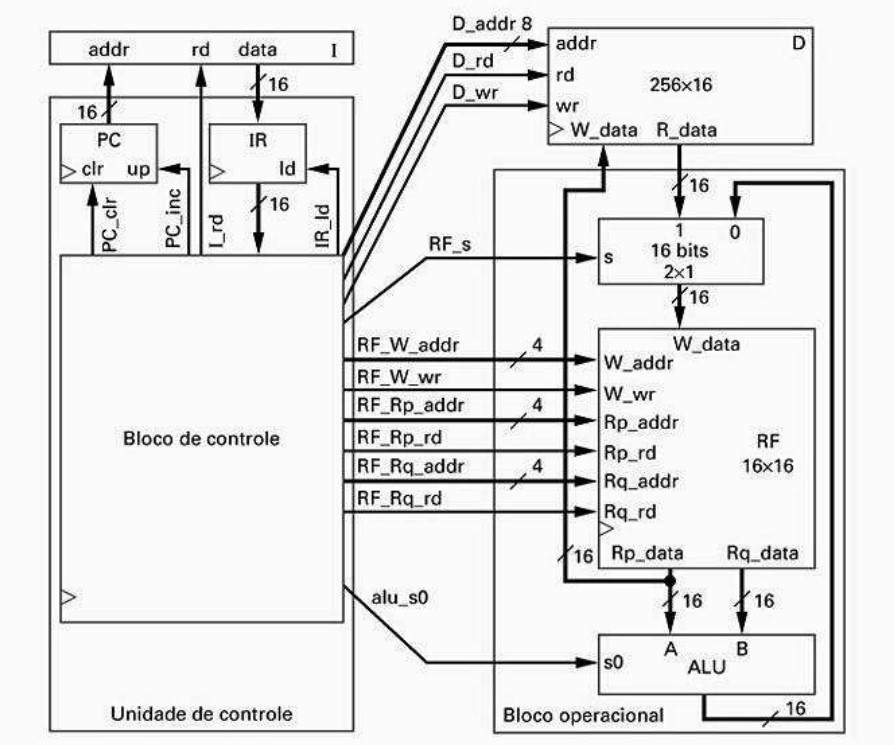
\includegraphics[width=1\textwidth]{operacionalecontrole3instr.jpg} 
    \caption{Unidade de controle e bloco operacional e interfaces entra ambos para um processador de três instruções.} 
    \label{fig:unidadeDeControleBlocoOperacional3Instr} 
     \hfill
\end{minipage}\hfill
\begin{minipage}{0.48\textwidth}
    \centering 
    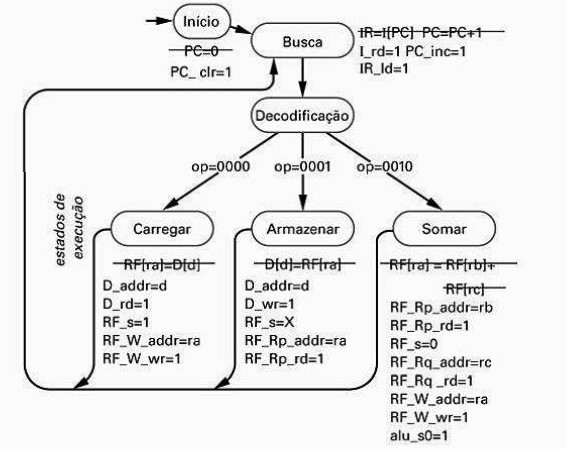
\includegraphics[width=1\textwidth]{fsmBaixoNivel3Instr.jpg} 
    \caption{FSM de baixo nível do processador de três instruções.} 
    \label{fig:FSMbaixonivel3instr} 
\end{minipage}
\end{figure}
 
Por cada instrução possuir 4 bits para endereçar o banco de registradores, ele dispõe de 16 registradores. Também, o bloco operacional tem um sinal de controle para a ALU(ULA) chamado alu\_s0. Quando alu\_s0=1, a ULA soma as duas entradas; quando alu\_s0=0, ela simplesmente deixa passar a entrada.
A memória de dados tem 256 palavras, uma vez que cada instrução possui 8 bits para endereçar a memória de dados.

Finalmente, podemos obter a FSM de baixo nível, substituindo as ações de alto nível pelas operações booleanas de saída, vista na figura \ref{fig:FSMbaixonivel3instr}.
 
Analisando o comportamento da FSM podemos ver como um programa seria executado nesta arquitetura de processador de três instruções:

\begin{boxlabel}
     \item A FSM naturalmente começa no estado Início, com $PC\_clr=1$, limpando o \textit{program counter} deixando-o em 0;
     \item No próximo ciclo de clock, a FSM entra no estado de busca, no qual lê a memória de instruções no endereço 0(porque $PC=0$) e carrega o valor lido em IR. Ao fim, incrementa o valor de PC. \textit{Algo como $IR[PC]=IM[PC]$};
     \item Em seguida, a FSM entra no estado de decodificação, sem ações realizadas, estando aqui para permitir que os valores dos códigos de operação se atualizem(as atualizações de registrador atribuídas a um estado só ocorrem de fato na próxima borda de clock). A depender dos 4 bits mais significativos do \textit{instruction register}, o próximo estado será carregar, armazenar ou somar;
     \item No estado de carregar, a FSM prepara as linhas de endereço de memória de dados utilizando os 8 bits menos significativos do \textit{instruction register} )($D_addr=d$) e habilitando a leitura da memória de dados($D\_rd=1$). Aqui, a seletora do multiplexador é ativada($RF_s=1$) para que o valor de saída da memória de dados vá para o banco de registradores. Finalmente, prepara o endereço de escrita do banco de registradores ($RF\_W\_addr=ra$), usando $IR[11...8]$ e habilitando a escrita ($RF\_W\_wr=1$). Tudo isso faz com que o conteúdo que esteja na memória de dados seja carregado no registrador apropriado do banco de registradores.
     \item De forma semelhante os estados Armazenar e Somar preparam as linhas de controle conforme a necessidade das operações de armazenamento e soma.
     \item Por fim, a FSM retorna ao estado de Busca, buscando pela próxima instrução.
\end{boxlabel}

\section{Processador programável de seis instruções}
Tendo em vista as limitações de um processador de três instruções, estendemos o conjunto de instruções do processador acrescentando mais três instruções.
Primeiramente, além das instruções vindas do processador de três instruções, \textit{load}, \textit{store} e \textit{add}, uma nova instrução permitirá carregar uma constante para um dos registradores do banco de registradores, permitindo novas operações como $RF[0]=RF[1]+5$, onde 5 é uma constante, ou seja,não se encontra na memória de dados.

Outra operação nova será a de subtração: similar à operação de soma já existente.

Finalmente, a sexta e última operação será a de "Saltar se zero". Esta instrução permitirá saltar para alguma parte do programa caso o conteúdo de algum registrador especificado for 0.

Expandindo nestas operações:

\begin{boxedd}
\begin{lstlisting}
Carregar constante - 0011(r3)(r2)(r1)(r0)(c7)(c6)(c5)(c4)(c3)(c2)(c1)(c0)
\end{lstlisting}    
Especifica que o número binário representado pelos bits $c_i$(conhecido como uma constante) deve ser deve ser carregado no registrador especificado pelos bits $r_i$. Aqui, $r_i$ corresponde à $IR[11...8]$ e $c_i$ corresponde à $IR[7...0]$. O mnemônico dessa instrução é:
\begin{lstlisting}
     MOV Ra, #c // RF[a]=c     
\end{lstlisting}
onde a pode assumir qualquer valor de 0 até $2^4 - 1$ em complemento de 2, ou seja, de 0 até 15, e c pode assumir qualquer valor entre $\frac{-2^8}{2}$ e $\frac{2^8-1}{2}$, ou seja, entre $-128$ e $+127$.
\end{boxedd}


\begin{boxedd}
\begin{lstlisting}
Subtrair - 0100(ra3)(ra2)(ra1)(ra0)(rb3)(rb2)(rb1)(rb0)(rc3)(rc2)(rc1)(rc0)
\end{lstlisting}    
Especifica a subtração dos conteúdos de dois registradores do banco de registradores especificados por $rb_i$ e $rc_i$. O resultando é então armazenado no registrador do banco de registradores especificado por $ra_i$(Lembrando que $ra$ corresponde $IR[11...8]$, $rb$ corresponde $IR[7...4]$ e $rc$ corresponde $IR[3...0]$). O mnemônico dessa instrução é
\begin{lstlisting}
     Sub Ra, Rb, Rc // RF[a]=RF[b]+RF[c]     
\end{lstlisting}
Os termos a, b e c podem assumir qualquer valor de 0 até $2^4 - 1$ em complemento de 2, ou seja, de 0 até 15. 
\end{boxedd}


\begin{boxedd}
\begin{lstlisting}
Saltar se zero - 0101(ra3)(ra2)(ra1)(ra0)(o7)(o6)(o5)(o4)(o3)(o2)(o1)(o0)
\end{lstlisting}    
Especifica que se o conteúdo do registrador especificado por $ra_i$ for 0, então carrega-se o PC com o valor atual de PC somado ao valor em oito bits e complemento de 2 $o_i$, podendo ser um \textit{offset} positivo ou negativo. Aqui, $ra_i$ corresponde à $IR[11...8]$ e $o_i$ à $IR[7...0]$. O mnemônico dessa instrução é: 
\begin{lstlisting}
     JMPZ Ra, offset // PC = PC + offset se RF[a]=0
\end{lstlisting}
Offset pode tomar qualquer valor entre $\frac{-2^8}{2}$ e $\frac{2^8 - 1}{2}$. Ou seja. podemos saltar para frente até 127 endereços ou para trás até 128 endereços. Aqui, também, onde a pode assumir qualquer valor de 0 até $2^4 - 1$.
\end{boxedd}
Resumindo, em um processador programável de seis instruções temos as seguintes instruções:
\begin{table}[h]
\centering
\caption{Conjunto de instruções de seis instruções}
\begin{tabular}{|l|l|}
\hline
\textbf{Instrução} & \textbf{Significado} \\ \hline
MOV Ra, d & RF[a] = D[d] \\ \hline
MOV d, Ra & D[d] = RF[a] \\ \hline
ADD Ra, Rb, Rc & RF[a] = RF[b] + RF[c] \\ \hline
MOV Ra, \#C & RF[a] = C \\ \hline
SUB Ra, Rb, Rc & RF[a] = RF[b] - RF[c] \\ \hline
JMPZ Ra, offset & PC = PC + offset \text{ se } RF[a] = 0 \\ \hline
\end{tabular}
\end{table}

Devemos também estender a noção da unidade de controle e bloco operacional para o processador de seis instruções)(figura \ref{fig:unidadeDeControleBlocoOperacional6Instr}). Primeiramente, a instrução de carregar constante necessita que possamos carregar o valor de $IR[7...0]$ no banco de registradores, além dos valores da memória de dados e da saída da ULA. Assim, aumenta-se o multiplexador do banco de registradores de 2x1 para 3x1, adiciona-se também mais um sinal de controle ao multiplexador e cria-se um sinal novo denominado RF\_w\_data que vai do bloco de controle se ligando à $IR[7...0]$ e entrano no multiplexador.

Segundo, a instrução subtrair requer que a ULA seja capaz de realizar a subtração. Então, adiciona-se um novo sinal de controle à ULA visando diferenciar quando fazer uma subtração e quando fazer uma adição, alu\_s1.


Por fim, a instrução saltar se zero requer a capacidade de detectar se um registrador é zero e somar $IR[7...0]$ ao PC. Assim, insere-se um componente no bloco operacional para determinar se a porta de leitura Rp do banco de registradores es´ta com todos os bits em zero. Também, modifica-se PC para que seja possível carregar $PC=PC+IR[7...0] \therefore PC=PC+offset$. Vale mencionar que o somador utilizado já subtrai 1 da soma, compensando o fato que o estado de Busca já incrementa 1 ao PC.

\begin{figure}[h!] 
    \centering 
    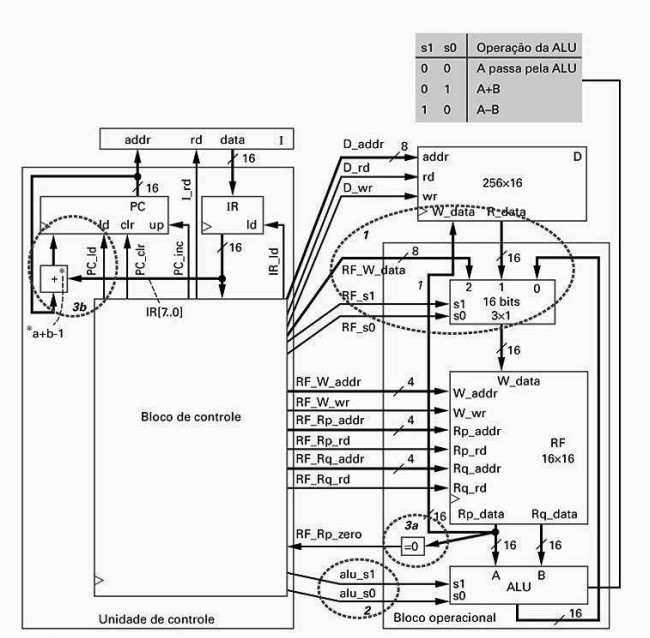
\includegraphics[width=0.5\textwidth]{operacionalecontrole6instr.jpg} 
    \caption{Unidade de controle e bloco operacional e
interfaces entra ambos para um processador de seis
instruções.} 
    \label{fig:unidadeDeControleBlocoOperacional6Instr} 
\end{figure}


Vamos estender também, naturalmente, a FSM do bloco de controle para lidar com as instruções adicionais. A figura
\ref{fig:fsmBaixoNivel6Instr} mostra seu diagrama:
\begin{figure}[h!] 
    \centering 
    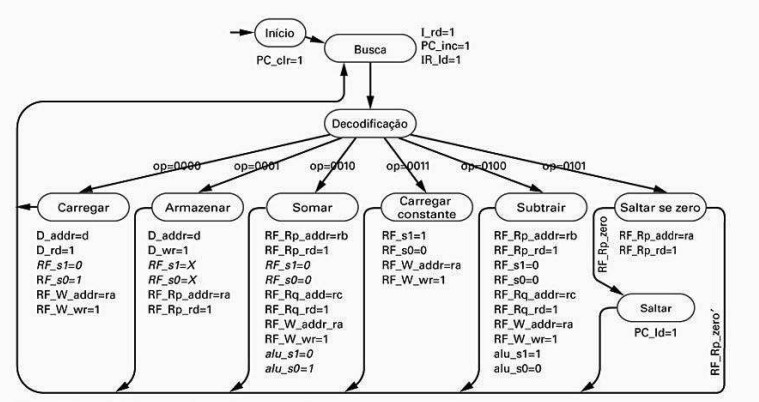
\includegraphics[width=0.7\textwidth]{fsmBaixoNivel6Instr.jpg} 
    \caption{FSM de baixo nível do processador de seis instruções} 
    \label{fig:fsmBaixoNivel6Instr} 
\end{figure}

Os estados início e busca permanecem os mesmos. Em decodificação, adiciona-se três novas transições para as três novas instruções. Também, os estados carregar, armazenar e somar sofreram alterações para refletir a necessidade do multiplexador do banco de registradores possuir duas variáveis de seleção e a ULA ser configurada com dois sinais. Além disso, foram adicionados os três estados extras:

\begin{boxlabel}
     \item No estado Carregar constante, configura-se o multiplexador do banco de registradores para deixar passar o sinal RF\_W\_data e o banco de registradores para escrever no endereço especificado por ra($IR[11...8]$);
     \item No estado Subtrair, executa-se as mesmas ações do estado Somar, exceto que a ULA é configurada para subtração ao invés de adição ($s1=1 $ e ($s0=0$);
     \item No estado de Saltar se zero, configura-se o banco de registradores para que o registrador especificado por ra seja lido e seu conteúdo colocado na port ade leitura Rp. Se o valor de Rp for composto apenas de 0s, então a saída RF\_Rp\_zero irá ser 1(e 0, caso contrário). Dessa forma, deve-se tratar de duas transições partindo do estado Saltar se zero. Se $RF\_Rp\_zero=0$, ou seja, o registrador lido(presente agora na saída Rp) não contém apenas 0s, a FSM volta para o estado Busca, ou seja, não ocorre salto. Se $RF\_Rp\_zero=1$, o registrador lido é composto só de zeros, então a FSM vai para o próximo estado, Saltar, na qual realmente ocorro o salto com o sinal de load do PC sendo 1($PC\_ld=1$).
\end{boxlabel}

\newpage
 


\end{document}
 